\documentclass[11pt]{article}
\usepackage{eacl2012}
\usepackage{times}
\usepackage{latexsym}
\usepackage{amsmath}
\usepackage{tikz}
\usepackage{graphicx}
\usepackage{multirow}
\usepackage{url}
\DeclareMathOperator*{\argmax}{arg\,max}
\setlength\titlebox{6.5cm}    % Expanding the titlebox

\title{Visualising Typological Relationships: Plotting WALS with Heat Maps}
%Title should perhaps be changed. 
% To?

% \author{Richard Littauer \\
% University of Saarland\\
% Computational Linguistics Department\\
% Saarbr\"ucken, Germany\\
%   {\tt richard.littauer@gmail.com} \\\And
% Rory Turnbull \\
% Ohio State University\\
% Department of Linguistics\\
% Columbus, Ohio\\
%   {\tt turnbull@ling.osu.edu} \\\AND
% Alexis Palmer\\
% University of Saarland\\
% Computational Linguistics Department\\
% Saarbr\"ucken, Germany\\
%   {\tt apalmer@coli.uni-sb.de}\\} 

\date{}

\begin{document}
\maketitle

% \begin{abstract}
% This paper presents a novel way of visualising linguistic typological data. Computational methods have only recently been applied in the formation and use of large typological databases. Many studies have since focused on discovering relations between languages using typology, often using sophisticated statistical techniques. However, few papers have provided new or newly applied ways of visually presenting the resulting data. Here, we show that one can use the data from the World Atlas of Language Structures \cite{wals-2011} to develop heat maps that can visually show the interconnected relationships between languages and language families. We hope that the images will bring a new perspective to the data, resulting in interesting findings and illuminating areas of research.
% \end{abstract}

\begin{abstract}
This paper presents a novel way of visualising relationships between languages. The key innovation of the visualisation is that it brings geographic, phylogenetic, and linguistic data together into a single image, allowing a new visual perspective on linguistic typology. The data presented here is extracted from the World Atlas of Language Structures (WALS)~\cite{wals-2011}. After pruning due to low coverage of WALS, we filter data about linguistic structures and attributes by geographical proximity in order to get at areal typological effects. The data are displayed in heat maps which reflect the strength of similarity between languages for different linguistic aspects. Finally, these are annotated for language family membership. The images so produced allow a new perspective on the data which we hope may facilitate interesting findings and perhaps even illuminate new areas of research.
\end{abstract}

%% This outline is just a suggestion. Feel free to mix it up as much as you want if you feel it would or should be better another way. 

\section{Introduction}

This paper presents a novel way of visualising relationships between languages. Relationships between languages can be understood with respect to linguistic features of the languages, their geographical proximity, and their status with respect to historical development. The visualisations presented in this paper are the first to bring together these three perspectives into a single image. One line of recent work brings computational methods to bear on the formation and use of large typological databases, often using sophisticated statistical techniques to discover relations between languages \cite[among others]{cysouw2011,daume07implication,daume09areal}, and another line of work uses typological data in natural language processing \cite[for example]{georgi:etal:10,lewis:xia:08}, but we are unaware of any previous approaches to visually presenting the resulting data.
%However, few papers have provided new or newly applied ways of visually presenting the resulting data. 
Here, we address this gap by using data from the World Atlas of Language Structures \cite{wals-2011} to develop heat maps that can visually show the interconnected relationships between languages and language families. 

%\item brief history of typology
The main envisioned application of our visualisations is in the area of linguistic typology. Typology has been used to derive implications about possible languages, and about the ordering of the human mind. Different theorists have taken different views on the relationship between typology and the universality of languages. For example, Greenberg \shortcite{greenberg}, a foundational work in the field, identifies a number of cross-linguistic typological properties and implications and aims to present them as truly universal -- relevant for \textit{all} languages. In a similar vein, typological universals have been employed as evidence in a generative story regarding language learning \cite{chomsky}.
% and claiming that they represented universals of grammar, and that they would hold true for all languages. In %a similar vein, Chomsky \shortcite{chomsky}%Check citation, make sure it is a good one
%has argued as a generativist that typological universals show that language is clearly an artefact of constraints involved with the learning process, and that some typological features are impossible due to this. 
Taking a different perspective, Dunn {\it et al} (2011) %Find citation
% The citation style you're using here is confusing me. Why not just \cite{chomsky} etc?
% Because that would be (chomsky, 2011). For inline ones, we need this.
% AP: changing these to \shortcite{chomsky}, which is only slightly more efficient, but slightly so.
argued that a language's typology relies upon the previous generations' language more than on any biological, environmental or cognitive constraints, and that there are pathways which are generally followed in language change based on the previous parent language. What these arguments have in common is a reliance on a view of linguistic typology that is potentially restricted in its scope, due to insufficient access to broad-scale empirical data, covering many features of many languages of the world. 

%Outside of the scope of theory, language typology is useful for other reasons. %Cite Xia and Lewis, MT, NLP, etc....

%\item WALS
The most comprehensive computational resource for linguistic typology currently available is the World Atlas of Language Structures (WALS).\footnote{As of 2008, WALS is browsable online (\url{http://www.wals.info}).}  WALS is a large database of details of structural properties of several thousand languages \cite{wals-2011}. The properties were collected from descriptive sources by the project's 55 authors. 
%Cut out stuff from here, moved it to Material and Methods. May not have been advised. 
However, for the several thousand languages in WALS, there is only about 16\% of the possible features filled---the data are \emph{sparse}, and the sparsity of the data of course make it difficult to perform reliable statistical analysis. One way to work around this limitation is to seek meaningful visualisations of the data in WALS, instead of simply relying on raw numbers. This is our approach. 

%In this paper:
In this paper, we will first discuss more fully our starting data, before going on to discuss the problems with analysing this data and how our methodology dealt with them. We will then present several graphs that highlight the possibilities of graphing WALS data. 

\section{Aspects of the Visualisations}

The visualisations described here bring together three types of information: linguistic features, geographical distance, and phylogenetic distance. For the current study, all three types of information are extracted from the WALS database. In future work, we may explore the use of alternate sources such as Ethnologue \cite{ethnologue} or MultiTree \cite{multitree} for alternate phylogenetic hierarchies. 

% The above sentence is vague. 16% of what? What does it mean for the features to be filled? Only 16% of the features are "full"? Only 16% of languages have full descriptions for each feature?

Dealing with sparse data is a computational problem, as any statistical information drawn from the database will, to a large extent, be an artefact of the database. For instance, if half of the languages were marked as having uvular stops (unlikely), and then in reality if all other languages not in the database had uvular stops, then the knowledge we would glean from the database would be significantly false and misleading. Given that there are around 6,000 languages in the world, the amount of languages on WALS means that this is a serious concern. Many researchers in recent years have been developing work-arounds for sparse databases; often because languages with low resources have a similar problem. %Cite cite cite

% The above para is also unclear. The sparsity of data problem just sounds like a sampling problem, which is endemic to all of science. Also, can we state at some point *how many* lgs are in WALS? that's not clear.

A solution to dealing with this issue is to visualise the data in WALS, instead of relying on raw numbers.

%Alexis [filler][filler]

%\item visualisation
%\item what visualisation can do for us
%\item Heat Maps  where they come from, what they are doing here


\subsection{Linguistic features}
\subsection{Geographic distance}
We measured geographic distance by choosing an arbitrary radius that would would create a decision boundary to cluster $n$-nearest neighbours. For our purposes, we went with 500km, as this proved to provide sufficient examples to draw from from cleaned WALS data. We also measured distance by selecting an arbitrary lower threshold for languages in the general area, and printed the results if the amount of cleaned languages in the area was a certain percentage over the amount of languages in the area total as specified by WALS. This number is clearly under-representative of the amount of contact languages, as only half of the world's languages are present in WALS. This proxy was not as good at choosing specific, useful examples, as the $n$-nearest nieghbours, as the languages chosen were often too far away. 
%Haversine Formula - distance on a sphere (earth) http://en.wikipedia.org/wiki/Haversine_formula
% (Vincenty formula would be more accurate (as earth is not a 
% perfect sphere), but much more computationally intense for
% 2678*2678 comparisons.
%   http://www.codecodex.com/wiki/Calculate_Distance_Between_Two_Points_on_a_Globe#Python
%Note - reprint the data with this formula worked in, as it makes more sense than what you're doing at the moment.

\subsection{Phylogenetic distance}

Languages are related phylogenetically either vertically, by lineage, or horizontally, by contact. In WALS, each language is placed in a tree hierarchy that specifies phylogenetic relations. In the WALS data files, this is specified by linking at three different levels: family, such as `Sino-Tibetan', sub-family, such as `Tibeto-Burman', and genus, such as `Northern Naga', . % Provisional tree hierarchies were also drawn from Ethnologue \cite{ethnologue} and MultiTree \cite{multitree}, but due to the low amount of overlap between non-sparse WALS entries and the possible alternative hierarchies drawn from Ethnologue or MultiTree, only the phylogenetic relations from WALS were used.
% If we didn't use the ethnologue or multitree data, we don't need to mention it.
% Well, we did run it - I don't know, I feel like it's important to mention that it is a neg result for new results mapping to Ethnologue. I wish I had known this before, by reading it in some other article. 

%Information about Ethnologue scrape %provided by steven moran -need to get the details
The WALS phylogenetic hierarchies do not take into account language contact. For that, we used geographic coordinates, which are present on WALS, as a proxy for contact. 
%\item Longitude and latitude, and how it is measured
%Distance:
%    For each language, the distance has been calculated. Currently we have a
%    2678x2678 matrix, which is a little large.



\section{Material and Methods}
%\item Information about WALS data
\subsection{WALS}

%192 features in WALS
At the time of submission, there were 81,828 datapoints for 2,678 languages (an average of 28 per language). At least one feature, the most populated, had data for 1,519 languages. There were 144 different chapters, each containing values for different, related features. It can be seen easily from these numbers that the data on WALS is \emph{sparse}. Ignoring the fact that a language having certain features will cancel out the possibility or probability of others, that means that the WALS possible data is only 15.8\% represented in the database.

Drawing a heat map where only 16\% of the features are available would be of little use. There are two options for dealing with this: to collapse the feature values in some way, or to select for languages that have a higher percentage of data filled than the average language. We opted for the second choice, and \emph{cleaned}  the file until it contained only languages that had either 30\% as a lower bound, or 50\% as a higher bound, of all of their entries filled. This cleaned data was then used in the other functions.  

%\item Description of typological data
	%Insert example here. Probably. 
	
%    Relations are defined by features. A possibility is combining features, and
%    creating a feature similarity metric - for instance, aligning various types
%    of syntactic universals together. - THis has been done: Xia and Lewis, 2008


%\item Measuring Phylogenetic distance
%\item Measuring Geographical distance
%\item Combined map - %Should be possible - give distance equal weightings, find the aggregate. 


Each final list was then resorted, so that the source language was centered in the map. This was due to one of the primary issues with using distance on a two dimensional graph. On the one hand, we would want close languages to be close together on the heat map. However, given the source language Egyptian Arabic, this would mean that Zulu, Saami, Mohawk, and Japanese might all roughly be placed next to each other on the map. This also means that Japanese might be placed next to Mohawk, and Mohawk again next to Korean. This is not ideal, and was the main justification for limiting the sphere of possible geographical languages to a reasonable distance, given the data. 


%    We could sort them lattitudinally or longitudinally - consider the case of
%    a Dravidian language at the south of India. This would work well, here. Or
%    Patagonian. Japanese would work - but we don't have the dialect scales, so
%    this may not show us anything, especially not with WALS. This helps us in
%    forcing our hand to make smaller maps - say, 30 languages - instead of
%    massive ones. 

% 	Rory, can we do this?

% I'm not sure what you're asking if we can do - sorting by lat or long?
% Aren't we already sorted by distance to other lgs?

% Instead of centering the line, use the line that is furthest to a cardinal point, and then have all languages in a certain direction (Ssw to nnw) for instance - lined up next to it. This might be able to stop one of the major problems of the heat map. 

%\item Compiling python scripts, converting into R
All of the code was done either in Python, or in R. %How to include this? In a link to the git hub?
The code was not computationally intensive, and did not take more than a couple of minutes to run.

%\item Sorting R output

\section{Results} %Or visualisations?

\begin{figure}[h]
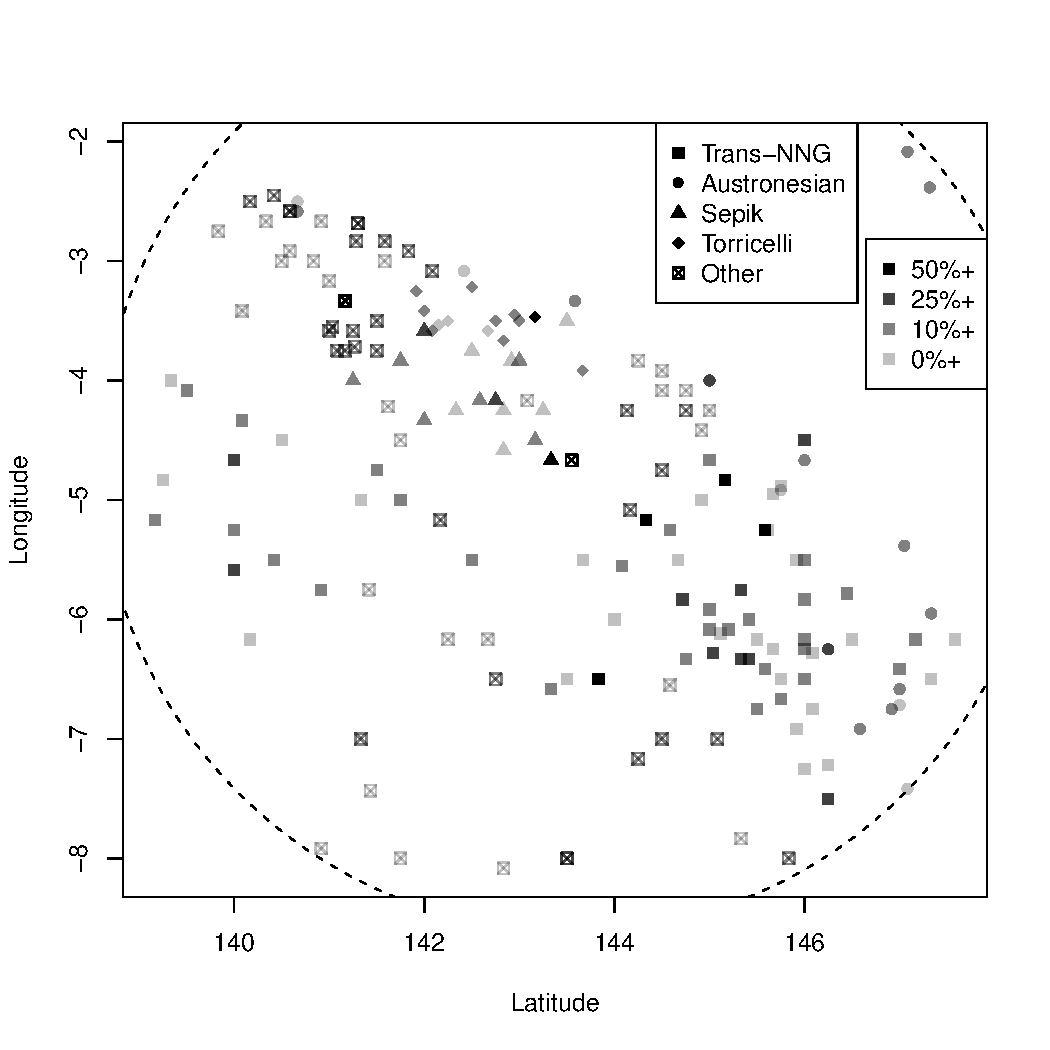
\includegraphics[width=3.1in]
{graph1.pdf} 
\caption{Sparse Data} 
\label{fig:sparse} 
\end{figure}

In Fig. \ref{fig:sparse}, we have plotted out the neighbouring languages for the most populous language area represented on WALS by longitude and latitude. The center language, Yimas, is a Trans New Guinean language, and is the center for the graph. The odd clustering is due to the Pacific Ocean - such geographical features limit the usefulness of distance as a measure. Another limit is the range of each language, which is not represented here, as each language is given only a single geographical coordinate that does not indicate the area over which the language resides, nor how many other languages coexist with it.

For each language within 500km, represented here by the dotted circle, the amount of features filled in WALS is shown. The majority have less than 50\% filled - there are only 171 such languages in WALS. This graph does not include languages not in WALS. It ought to be clear from this that the data in WALS is too sparse to draw immediate conclusions from, which furthers the need for visualizations. 



Lorem ipsum dolor sit amet, consectetur adipiscing elit. Mauris massa elit, facilisis quis elementum quis, tincidunt et massa. Suspendisse et lacus augue, sit amet molestie est. Aliquam luctus vestibulum tellus, nec consectetur elit porttitor ut. Aenean tellus velit, placerat ac placerat nec, ultricies quis nunc. Vivamus eget neque id diam posuere tincidunt ac vel nibh. Morbi vitae eros turpis. Vestibulum vitae nulla diam. Class aptent taciti sociosqu ad litora torquent per conubia nostra, per inceptos himenaeos.
\begin{figure}[h]
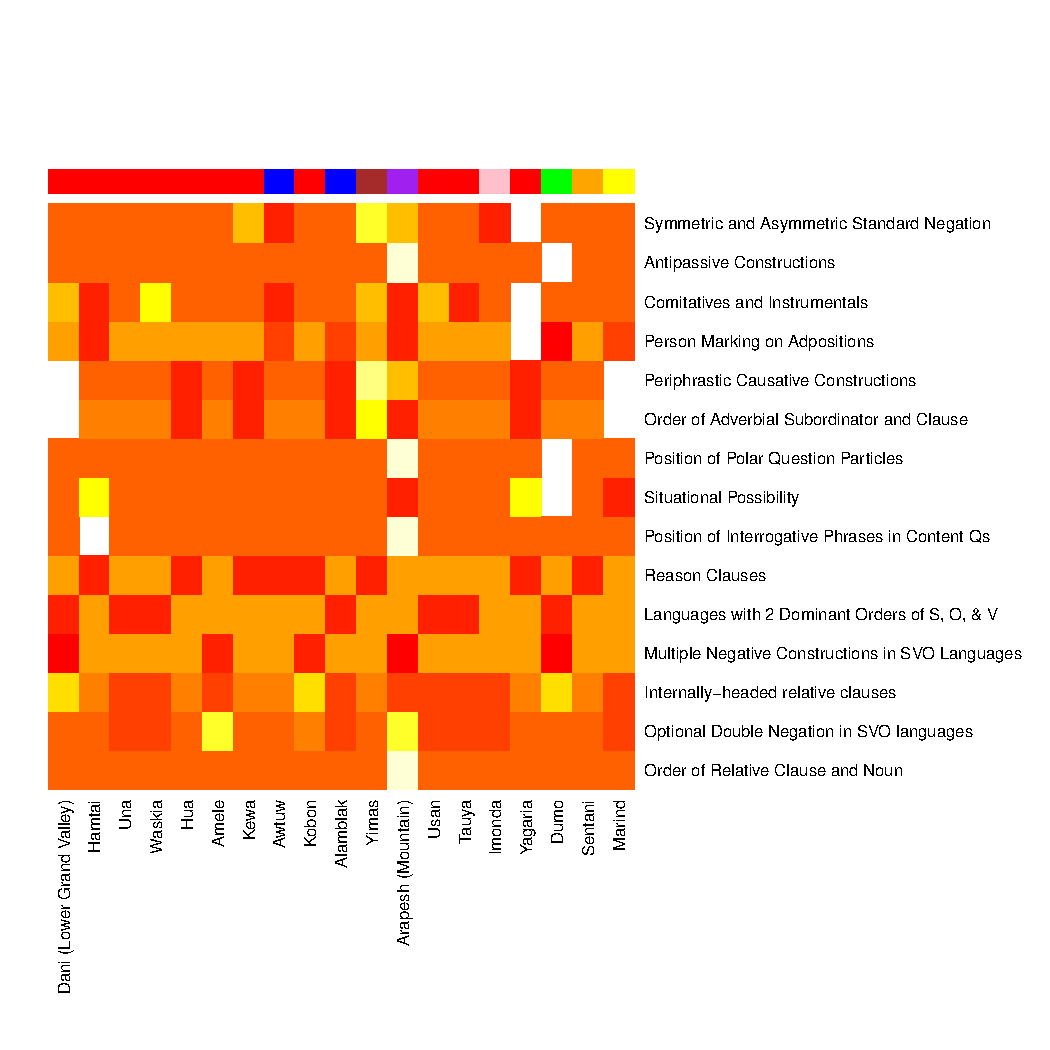
\includegraphics[width=3.1in]
{graph2.pdf} 
\caption{Example 1} 
\label{fig:sparse} 
\end{figure}
Vestibulum elit odio, luctus eget elementum a, interdum id sem. Cum sociis natoque penatibus et magnis dis parturient montes, nascetur ridiculus mus. Sed scelerisque est eget lorem eleifend vestibulum. Ut dui dolor, tincidunt ac fringilla vitae, mollis tristique ligula. Quisque urna tortor, venenatis eu bibendum id, condimentum vel neque. Lorem ipsum dolor sit amet, consectetur adipiscing elit. Sed at ligula nunc, et tincidunt mi. Donec pellentesque mauris rutrum odio vulputate a egestas neque mattis. Curabitur molestie adipiscing leo, sed posuere elit luctus id. Ut arcu diam, scelerisque at hendrerit eu, venenatis eget urna. Vestibulum ante ipsum primis in faucibus orci luctus et ultrices posuere cubilia Curae; Donec feugiat, tellus quis viverra porttitor, dolor dolor vehicula tortor, ac porta nisi elit non ante. Proin ligula odio, condimentum nec pellentesque a, cursus ac nulla. Cras aliquet magna ut dolor suscipit congue.

\subsection{Heat maps}
\begin{itemize}
\item Phylogenetic distance heatmaps
%only relevant ones, or ones that seem particularly useful. We should be making a few - world, region, etc. Going to need to make a supplement, perhaps. 
\item Geographical distance heatmaps
\item Combined maps
\end{itemize}


\section{Discussion}
\begin{itemize}
\item What these tell us (map by map)
\item What these tell us, overall - implications
\item Warnings: sparse data, data not there, etc. 
\item Future work 
%    We could also plot on a world map, but that would not be a heat map. An
%    option for this would be to color gradiantly based on certain featurs - for
%    instance, color could indicate phoneme size. 
%
%    Another option would be a matrix map of some sort - Again, not a heat map,
%    and beyond the scale of this current study.
\end{itemize}

\bibliographystyle{acl}
\bibliography{lingviz}

\end{document}
